\documentclass[SE,authoryear,toc]{lsstdoc}
% lsstdoc documentation: https://lsst-texmf.lsst.io/lsstdoc.html
\input{meta}

% Package imports go here.

% Local commands go here.
\newcommand{\FIXME}[1]{{\bf \textcolor{red}{#1}}}

%If you want glossaries
%\input{aglossary.tex}
%\makeglossaries

\title{Announcement of Opportunity: Community Engagement with Rubin Observatory Commissioning Effort}

% Optional subtitle
% \setDocSubtitle{A subtitle}

\author{%
Keith Bechtol, Chuck Claver, System Integration Test and Commissioning Team, Project Science Team, on behalf of the Rubin Construction Project
}

\setDocRef{SITCOMTN-010}
\setDocUpstreamLocation{\url{https://github.com/lsst-sitcom/sitcomtn-010}}

\date{\vcsDate}

% Optional: name of the document's curator
% \setDocCurator{The Curator of this Document}

\setDocAbstract{
The Vera C. Rubin Observatory invites members of the US and Chilean LSST science communities to join the Project Commissioning Team in order to make value-added contributions that facilitate an efficient transition into LSST Operations. In this Announcement of Opportunity (AO) we include descriptions of its purpose, examples of value-added contributions, terms and conditions for participation, and the process to respond to this AO via submitted Letters of Interest (LOIs).

The anticipated total value-added contribution via this program is of order 15-20 FTE of effort. This effort will likely be distributed across a larger number of individuals and preferably organized into discrete groups of like interests and skills, and performed over a roughly two-year period that includes calendar years 2022 and 2023. Financial support associated with this AO is limited, and non-Rubin-staff members of the Commissioning Team are generally expected to have other sources of support (limited travel and local accommodation support to enable on-site work at key activity centers in Tucson, SLAC, and Chile can be made available).
}

% Change history defined here.
% Order: oldest first.
% Fields: VERSION, DATE, DESCRIPTION, OWNER NAME.
% See LPM-51 for version number policy.
\setDocChangeRecord{%
  \addtohist{1.0}{2021-07-09}{Initial Release}{Keith Bechtol}
  \addtohist{1.1}{2021-07-22}{Update data release scenarios figure}{Keith Bechtol}
}


\begin{document}

% Create the title page.
\maketitle
% Frequently for a technote we do not want a title page  uncomment this to remove the title page and changelog.
% use \mkshorttitle to remove the extra pages

% ADD CONTENT HERE
% You can also use the \input command to include several content files.

\section{Executive Summary}

The Vera C. Rubin Observatory invites members of the US and Chilean LSST science communities to join the Project Commissioning Team in order to make value-added contributions that facilitate an efficient transition into LSST Operations. In this Announcement of Opportunity (AO) we include descriptions of its purpose, examples of value-added contributions, terms and conditions for participation, and the process to respond to this AO via submitted Letters of Interest (LOIs).

The anticipated total value-added contribution via this program is of order 15-20 FTE of effort. This effort will likely be distributed across a larger number of individuals and preferably organized into discrete groups of like interests and skills, and performed over a roughly two-year period that includes calendar years 2022 and 2023. Financial support associated with this AO is limited, and non-Rubin-staff members of the Commissioning Team are generally expected to have other sources of support (limited travel and local accommodation support to enable on-site work at key activity centers in Tucson, SLAC, and Chile can be made available).

\section{Purpose}
\label{purpose}

The Rubin Observatory Construction Project is entering its system integration and commissioning phase. The Project seeks to enhance the capabilities of the existing Commissioning Team by inviting US and Chilean members of the science community to work directly alongside Rubin Observatory staff as members of the Commissioning Team on specific tasks that will accelerate and enhance an efficient transition to LSST operations. Our goal with this AO is to integrate expertise from the community to enhance and diversity of the Project's planned commissioning effort and thereby provide added value. The anticipated total value-added contribution via this program is of order 15-20 FTE of effort. This effort will likely be distributed across a larger number of individuals and preferably organized into discrete groups of like interests and skills, performed over a roughly two-year period that includes calendar years 2022 and 2023 (this will apply to Builder status). Eligibility and group organization are discussed in Section~\ref{eligibility}. Examples of added-value contributions are listed in Section~\ref{examples}. This joint effort between Project staff and community will help provide a deeper understanding of the performance and characteristics of the Rubin Observatory as it enters into the operations phase.

This AO has a distinct focus from other interactions between Rubin Observatory and the science community around commissioning data. The Rubin Operations Team plans to provide access to commissioning data prior to the first formal LSST Data Release (DR1) in the form of a series of Data Previews (DPs; Appendix~\ref{data_previews}). The Data Previews are intended to provide access to commissioning data for US and Chilean scientists and international LSST data rights holders (the LSST science community) to help them prepare for science and to provide technical and scientific feedback to Rubin Observatory, as well as to provide practice for the Operations Team to prepare and support major data releases. In contrast, this AO is issued by the Rubin Construction Project and defines a mechanism for making specific value-added contributions to the commissioning effort on a more rapid timescale in direct collaboration with Rubin Observatory staff as members of the Commissioning Team. The deep level of engagement described in this AO comes with specific rights and responsibilities, as outlined in Section~\ref{rights_responsibilities}. Working in the Commissioning Team offers direct experience with and deep understanding of the full chain from observations to final data products and data access tools that will be released to the science community, including the hardware, image properties, and Science Pipeline algorithms. Through their efforts, the new members will be contributing to the readiness of Rubin Observatory to deliver its science products to the global Rubin community. 

The Project will not rely on the contributions from non-Rubin-staff team members to fulfill core construction requirements and operational readiness criteria. The intent for these contributions is to add value to the commissioning effort as given by examples below.  No papers presenting novel scientific results may be posted/submitted by anyone before the associated Data Preview release date. The focus of the commissioning effort is on demonstrating operational readiness rather than realizing scientific discoveries with the commissioning data itself.

\section{Examples of Value-Added Contributions}
\label{examples}

The Rubin Construction Project is scoped and has been planned to verify the set of system-level requirements listed in the LSST System Requirements \citedsp{LSE-29} and Observatory System Specifications \citedsp{lse-30} documents, and to demonstrate operational readiness as defined in the Construction Completeness and Operational Readiness Criteria \citedsp{SITCOMTN-005}. 

The following set of examples of value-added contributions to the commissioning effort are intended to guide the preparation and evaluation of Letters of Intent (LOIs). When preparing the LOIs, please mention the specific areas of intended effort. 

This list is not exhaustive. Additional value-added contribution areas may be possible and these concepts should be included in an initial indication of interest (see timeline) to allow iteration with the Project prior to the final LOI submission.

\subsection{Example Contributions Sought with this AO}

\textbf{Example 1: Investigation and mitigation of sensor anomalies for ComCam and LSSTCam detectors} using calibration and on-sky data.

\textbf{Example 2: Contributions to the integration, testing, and scientific validation of calibration systems} such as the Auxiliary Telescope (AuxTel), Collimated Beam Projector (CBP), and Multi-site All-Sky CAmeRA (MASCARA).

\textbf{Example 3: Absolute photometric calibration.} Includes connecting external observations, modeling, and synthetic photometry with Rubin Observatory observations of  spectrophotometric standards. Includes utilizing other surveys to investigate the calibration of the internal LSST photometric system relative to an external absolute scale.

\textbf{Example 4: Technical and scientific analyses of on-sky commissioning data to inform the initial LSST observing strategy} -- in particular, the optimization of dithers in the Deep Drilling Fields and Wide Fast Deep survey, evaluation of two snaps versus one snap in a visit, exploring technical constraints of specialized survey modes, etc.  For example:
\begin{itemize}
\item Given two dither patterns evaluate the systematic limits of key parameters -- which dither patterns would suppress instrument artifacts such as scattered light and internal optical glints.
\item Explore cadence optimization in less than ideal (e.g. bright time) conditions
\item Cadence optimization during twilight at the beginning and end of night
\end{itemize}
This effort is of a more tactical / technical optimization / fine-tuning nature and is distinct from the strategic planning underway through the \href{https://www.lsst.org/content/survey-cadence-notes-2021}{Cadence White Paper} effort and \href{https://www.lsst.org/content/charge-survey-cadence-optimization-committee-scoc}{Survey Cadence Optimization Committee} (SCOC).

\textbf{Example 5: Anomaly analysis of the Engineering Facility Database.} This example analysis is meant to apply Machine Learning/Deep Learning and other AI or statistical approaches to search for otherwise undetected anomalies in the system performance and telemetry and correlate these with properties of the image data and catalog parameters.
 
\textbf{Example 6: Extended analysis to characterize system performance at the margins of operational parameter space.} Over the course of commissioning the Telescope and Camera will be operated over a wide range of environmental conditions. This example analysis is meant to characterize the multiple performance metrics, of both scientific and technical types, and to correlate these metrics with environmental parameters (e.g., atmospheric seeing, sky brightness, humidity, outside temperature, wind speed and direction).
 
\textbf{Example 7: Evaluation of operational configurations of the observatory to determine optimum performance.} The Rubin Observatory has been designed with many degrees of freedom built in, in order to optimize system performance responding to different observing conditions. This example is meant to explore and analyze the optimal operational parameters (e.g., mirror support systems, telescope mount dynamics, camera electronics, dome wind screen, in-dome temperature control) to determine the appropriate configurations and procedures in the multi-dimensional parameter space for the as-built system.

\textbf{Example 8: Development of image and catalog visualization tools,} including capability to interactively explore and ``drill down'' into the data. Full focal plane image visualization. Visualization of telemetry and trending of technical and scientific performance. Contributions in this area could potentially expand upon, use and be implemented within the planned functionality of the Rubin Science Platform.

\textbf{Example 9: Algorithm development and testing for the Rubin Science Pipelines,} specifically instances where Rubin Data Management is implementing algorithms into the science pipelines that are being collaboratively developed with the community. Contributions in this topic could include testing, iterative development, and optimization of parameters using on-sky data for such algorithms.

\textbf{Example 10: Science validation and characterization of object detection, deblending, and interaction with background modeling.} This includes but is not limited to:
\begin{itemize}
\item Effects of ghost light from bright stars on faint stellar photometry and galaxy shape estimation
\item Effects of diffuse scattered light on faint stellar photometry and galaxy detection
\item Impacts of variable image quality on object detection, deblending, and measurement
\item Crowded field photometry
\item Preservation of low surface brightness objects in the data processing
\item Characterization and impacts of Galactic cirrus
\end{itemize}

\textbf{Example 11: Science validation of stray and scattered light mitigation and modeling,} including interactions with background modeling and the detection/photometry of low surface brightness features. For example, develop a predictive numerical model of ghost images from a bright source at an arbitrary position in the full field of view to reduce background modeling systematics.

\textbf{Example 12: Science validation of template generation and difference imaging.} Photometric accuracy of difference image analysis in complex environments and across a range of observing conditions. Studies of the variation of performance with respect to properties of templates. Validating the detection and measurement of known transient, variable, and moving objects.

\textbf{Example 13: Science validation using survey metadata maps.} Includes geometric survey coverage and survey property statistics represented as spatial maps over the observed footprint.  Maps and analysis will be done using existing Rubin Observatory software or extensions thereof.  Part of this work will include the validation of sky maps of distributions of environmental conditions during observations, data properties, along with computed performance metrics.

\textbf{Example 14: Observing support.} Contributions to daytime and nighttime summit operations; optimization and documentation of processes and procedures. See prerequisites and expectations described in Section~\ref{chile}.

\textbf{Example 15: Developing user-oriented documentation of science pipelines, data access services, and operational procedures,} including the development of tutorials through the Rubin Science Platform.

\textbf{Other:} Additional scientific validation and characterization studies that will improve understanding of the as-built system and enhance early operations are invited. Proposals of this type should specifically address the timeliness of the value-added contribution and relevance for advancing the operational readiness of Rubin Observatory.

\subsection{Ex Officio Members of the Commissioning Team}

In this section, we describe several categories of non-Rubin-staff members of the Science Community who will automatically become members of the Commissioning Team in order for them to more efficiently carry out responsibilities associated with their designated roles. Individuals in these categories do NOT need to respond to this AO. Contributions from Ex Officio members of the Commissioning Team do not count toward the envisioned 15-20 FTE of effort associated with this AO. 

Members of selected Commissioning Alert Broker Teams. Alert brokers are third-party services provided by the community. While Rubin is not responsible for the commissioning of the brokers, Rubin staff will work with the five or more selected broker teams to ensure that they can be commissioned and are ready for receiving and distributing the LSST alert stream at the start of LSST operations.  All members of the five selected broker teams automatically become Commissioning Team members.

Members of the selected photometric redshift teams. These members guide implementation and perform science validation for photometric redshift estimators. All members of the selected photometric redshift teams automatically become Commissioning Team members. See \citeds{dmtn-049} for the roadmap for selecting and validating one or more photo-$z$ estimators for the LSST Object catalog.  

Members of the Survey Cadence Optimization Committee (SCOC) will become members of the Commissioning Team in order to synthesize technical input and guide analyses that will inform decisions regarding the initial LSST observing strategy. 

International In-kind Contributor Teams with responsibilities directly related to commissioning will automatically become members of the Commissioning Team.

Groups who have already been performing work directed by the Project under collaborative or contracted efforts and who have made material contributions to construction effort will continue to be members of the Commissioning Team. 

\section{Terms and Conditions for participation in the Commissioning Team}
\label{terms}

Participation as a Commissioning Team member will be based on assessed value-added and capabilities to complement the existing Rubin Observatory Commissioning Team. By its nature, commissioning a complex system like the Rubin Observatory comes with many unknowns, therefore it is required that the team remain flexible in their assignments as the commissioning process unfolds. 

The Project reserves the right to decline any group's or individual's offer for any reason.  The Project can decide to terminate a group's or person's role on the team status at any time due to poor performance or undue overhead. The Project will not rely on the contributions from non-Rubin-staff team members to fulfill the core commissioning requirements to the Operations Readiness Review and the federal funding agencies. Non-Rubin-staff Commissioning Team members will be providing value-added contributions to extend the basic commissioning scope.

Financial support associated with this AO is limited, and non-Rubin-staff members of the Commissioning Team are generally expected to have other sources of support. Limited support for travel to enable on-site work in Chile, Tucson, and at SLAC can be made available.  Funds can also be made available to support accommodations while work is conducted at the Chile Summit site. Specifics will be negotiated on an individual basis.

\subsection{Rights and Responsibilities}
\label{rights_responsibilities}

\begin{enumerate}

\item Science Community members who become members of the Commissioning Team via this AO will have the opportunity and the expectation to collaborate directly with the Project staff on Rubin commissioning efforts, together with all the associated work experience and training opportunities entailed, as well as potential to enhance the scientific reach of LSST data for the benefit of the broad Rubin community. Participants agree to conduct work assignments from the Project with a defined scope and schedule for delivery. These work assignments will be ``value-added" contributions with respect to Project requirements from the federal funding agencies for Operations Readiness (see examples in Section~\ref{examples}). Each non-Rubin-staff member/group of the Commissioning Team will be assigned a functional point of contact within the Project to help integrate their efforts.

\item Submitted LOIs (Section~\ref{loi}) will be used as the basis for formally signed agreements (Memoranda of Understanding; MOUs) between the Rubin Observatory Construction Project and each individual/group that is selected to participate in commissioning activities. The MOUs will be assessed and re-evaluated on a yearly basis to ensure that the goals and responsibilities of both the Project and the participants are being met. 

\item All Commissioning Team members will have full unfettered access to all commissioning data products as soon as they are acquired. 

\item All members of the Commissioning Team agree to a set of publication policies (Section~\ref{publications}). In particular, no scientific publication based on the commissioning data shall be made prior to that data being released to the science community.  Technical publications will be allowed (see below). All Commissioning Team members are eligible to become co-authors on publications to which they contribute, including the series of planned Rubin Observatory Construction Papers.

\item Contributions to the commissioning effort performed under the direction of the Project count towards the attainment of Builder status \citedsp{RDO-013}.

\item Commissioning Team members are expected to use approved Project tools and processes for communication, data access and analysis, documentation, software development, work management, etc. For example, nearly all high-level science analysis tasks will use Python programming language, and many will make use of the Rubin Software Stack and Rubin Science Platform. Training opportunities will be provided by the Project to increase proficiency with these tools. 

\item All source code created by Rubin Observatory Data Management is publicly-available open source and carries an Open Source Initiative (OSI)-approved license. All software developed for the commissioning effort is expected to follow the Project's open source policy. There may be some situations in which science validation analyses making use of private software developed outside the commissioning context are deemed sufficiently valuable to the commissioning effort that an exception may be granted by the Project Director. 

\item Depending on their assigned task(s), some participants may be expected to spend extended periods at one of three primary Rubin Observatory sites: 1) Chile -- either La Serena and/or Cerro Pach\'{o}n (see additional requirement below); 2) Rubin Observatory offices in Tucson; and 3) the US Data Facility located at SLAC. In addition, participants will be invited to attend periodic workshops, bootcamps, and/or meetings for training and focused working sessions. It is expected that remote participation in these events will also be possible in cases where the work can be completed remotely.


\item The typical expected commitment for non-Rubin-staff members of the Commissioning Team is roughly 0.2 to 0.5 full time equivalent (FTE) averaged across the members of collaborating groups over the calendar years 2022 and/or 2023. For university faculty, this expected level of commitment should be interpreted as roughly 20\% of research time during these years. The exact timing of effort might be variable according to needs to respond to emergent issues. 

\item Members of the Commissioning Team are expected to follow guidance regarding types of internal communications and information that may be shared with the wider Rubin community.

\item All members of the Commissioning Team are expected to follow \href{https://www.lsst.org/scientists/codes-of-conduct}{professional standards of conduct} adopted by the Project.

\item Science validation and characterization investigations during commissioning are specifically intended to optimize operational efficiency of the observatory, and to enhance delivered data quality of the Data Previews and LSST DR1. Members of the Commissioning Team should strive for collaborative and collegial interactions that benefit the entire Rubin Community, and to recognize the contributions of the many individuals that have contributed to the Project. 

\end{enumerate}

\subsection{Requirements for working on-site in Chile}
\label{chile}

It is expected that most Commissioning Team members will conduct data analysis tasks from sites other than the Rubin Observatory site in La Serena and the Cerro Pachon summit. Working on-site in Chile is intended for individuals working directly with hardware or observation support. 

Key criteria for working on-site in Chile:
\begin{itemize}
\item Demonstrate a working understanding of the observing systems in Chile including but not limited to:
	\begin{itemize}
	\item Observatory Command-Control interface and scripting (Python based)
	\item Observational constraints given current environmental conditions
	\end{itemize}
\item Commit to providing 3 months remote observing support prior to scheduled time in Chile
\item Willingness and ability to spend at least 3 months in Chile to support on-site observations and technical activities both on the Summit and in La Serena. This includes extended continuous periods (e.g. week or more) at the Summit Facility.
\end{itemize}

\subsection{Group management and accountability}

Each group responding to this AO will have designated a group leader who is the primary point of contact to the Rubin Observatory Project. The group leader is responsible for management of the group and for the timely completion of assigned tasks (see Section~\ref{eligibility}). Given potential emergent issues encountered during commissioning, and the nature of some value-added contributions as active research topics, completion of value-added contributions is intended to be on a ``best-effort'' basis as the research allows. While on-boarding and task-specific training and guidance will be provided, together with access to Project communication tools and documentation resources, the Project is only able to provide limited one-on-one training and support for non-Rubin-staff members of the Commissioning Team. Participating individuals/groups should plan to prepare as needed for their specific contributions.

Participants in this AO program will be assigned to one or more teams within the larger commissioning effort, and the individuals and/or groups will be assigned a functional point of contact within the Project to help integrate their efforts.

\subsection{Publication policy statement for using commissioning data}
\label{publications}

All members of the Commissioning Team will follow the publication policies of the Rubin Observatory Project, including the Rubin Data Policy \citedsp{RDO-013} and Rubin Project Publication policy \citedsp{LPM-162} as they apply to commissioning data.

\textbf{No papers presenting novel scientific results may be posted/submitted by anyone before the associated data release, which for commissioning data means the relevant Data Preview release date.} The Project has authority to determine the classification of technical versus scientific papers prepared by members of the Commissioning Team. Rubin Observatory reserves the right to sanction Users who violate this policy, as described in the Rubin Data Policy \citedsp{RDO-013}. 

The Project has planned a series of Rubin Observatory Construction Papers to describe the technical and scientific performance of the as-built system. The preparation of these papers follows the Rubin Project Publication policy. All members of the Commissioning Team are eligible to be co-authors on Rubin Observatory Construction Papers to which they contribute. The planned scope of the Construction Papers is limited to technical and scientific performance evaluation; the Construction Papers are not intended to present novel scientific results.

The Rubin Data Policy \citedsp{RDO-013} defines proprietary data products and derived data products. No proprietary data products from commissioning may be shared outside the Commissioning Team prior to the associated data release without explicit approval. The Project will define a process to approve the sharing of derived data products based on commissioning data prior to the associated data release. Any such derived data products approved for release must be presented in public forums accessible to the entire science community. There will be periods of commissioning for which specific types/subsets of proprietary as well as derived data products are embargoed and cannot be shared outside the Commissioning Team. Specific policies regarding informal communications beyond the Commissioning Team will be provided by the Project; guidance may evolve throughout the commissioning period. 

All investigations of commissioning data are considered to be open to the entire Commissioning Team. Members of the Commissioning Team are welcome to initiate and contribute to additional technical papers based on commissioning data beyond the planned set of Construction Papers. Additional technical papers using commissioning data products that are submitted and/or posted prior to the associated Data Preview release date must follow the Rubin publication policy. Following the Data Preview release date, additional technical papers using internal information, data products, and/or tools that are not included in released Data Previews continue to follow the Rubin Publication Policy. The scope of these additional papers should complement the scope of the Construction papers.

Science papers using only Rubin Observatory data from the released Data Previews follow the Rubin Data Policy \citedsp{RDO-013} and do not go through the Rubin Project publication process. For papers that substantially benefited from interactions with the Commissioning Team, authors are encouraged to invite contributing individuals to join as co-authors, as per the Rubin Publication Policy.

\section{Responding to this AO}
\label{loi}

\subsection{Eligibility and Group Organization}
\label{eligibility}

All members of the Rubin Observatory data rights community from the US and Chile \citedsp{RDO-013} are eligible to respond to this AO via submitting a Letter of Intent (LOI). There was a separate process for International LSST Data Rights and In-kind Contributions that included contributions to Rubin Observatory commissioning.

Collaborating individuals are encouraged to submit a single LOI for their group in response to this AO. The groups may be multi-institutional. The groups may include individuals across a range of career stages. Each group must identify a leader who will serve as the primary point of contact with the Rubin Observatory Project. The group leader will ensure that tasks assigned to their group are advancing and completed on the schedule set by the Project and that the work meets the standards defined by the Project. The group leader is responsible for the day-to-day management and advising of their group (or for delegating this responsibility within the group). For each group member who does not have Principle Investigator status or is not independently funded, a supervisor responsible for their employment must sign-off on their participation in the Commissioning Team at the time of formalizing the agreement between the Rubin Project and the participating individuals.

During the process of LOI preparation and evaluation, the Project may suggest reorganization of groups (e.g., merging related efforts or breaking up large groups) to increase efficiency.

\subsection{Timeline for Letter of Interest (LOI) submission and evaluation}

\begin{itemize}
\item \textbf{AO release:} 9 July 2021
\item \textbf{Indication of interest via web form:} 6 August 2021 (optional)
\item \textbf{Project Community Workshop - QA Session and ``office hours'':} 9-13 August 2021
\item \textbf{Project response regarding indication of interest:} 31 August 2021
\item \textbf{Final LOI submission:} 1 October 2021
\item \textbf{Project response to LOIs and formalization of agreements:} December 2021
\item \textbf{Engagement with Commissioning Team begins:} first quarter 2022
\end{itemize}

The Project considers this AO as stated as a one-time cycle for engagement by the US and Chilean communities. If the need and/or opportunities present themselves, the Project may issue a similar second Announcement of Opportunity in 2022. 

\subsection{Indication of Interest}

Groups/individuals considering to submit an LOI are invited to indicate their intent via a brief \href{https://forms.gle/fu5WsRgEYewbSvs76}{webform}. The Project will collect these submissions and provide brief feedback to the groups/individuals. 

\subsection{Elements for a Letter of Interest (LOI) response to this AO}

Letters of Interest (LOI) should address the following topics under separate section headings. An LOI template is provided \href{https://docs.google.com/document/d/12mYS3H0xRZme2t0leGIHfzwNgh575QhqsVnoUz7ybqQ/edit?usp=sharing}{here}. The expected length of an LOI is roughly 2-3 pages; more space might be warranted for larger groups and/or those with multiple proposed contributions. 

\begin{enumerate}
\item Name and contact information for the group leader

\item Statement of interests and proposed contributions. Please be as specific as possible, indicating the specific area(s) from the set of example contributions listed in Section~\ref{examples}. Proposed contributions must correspond to one or more of the examples, or explicitly label the contribution as type ``Other''. Plans to use private software that is not publicly released under an open source license must be specifically mentioned.

\item Statement of core competencies and adaptability
\begin{itemize}
\item Please mention current and previous engagement with the Rubin Observatory Project and/or LSST Science Collaborations, experience with and/or contributions to the Rubin Science Pipelines, and familiarity with hardware and/or software components of the Rubin Observatory system.
\item Please mention expertise, experience, prior work relevant to the specific intended area(s) of contribution.
\end{itemize}

\item Summary of personnel involved. For each individual, please include institution, career stage, FTE availability for Rubin commissioning related work in calendar years 2022 and 2023. 

\item Description of any support and resources available to each individual if they are necessary to complete their contributions and plans (e.g., salary/stipend, travel and local accommodation). Note that analysis of commissioning data is expected to be done using Project computing resources.

\item Description of any additional resources that are needed to fulfill your proposed contributions. To support this AO, the Project has limited funding for travel to and local accommodation at key activity centers: Tucson, Chile and SLAC.  Regrettably, the Project does not have funding for stipend or supplemental salary support.

\item Rubin is committed to providing opportunities for diverse and traditionally underrepresented groups. Please indicate how your proposed contribution will align with this commitment, for example, intent to provide training experience to early career scientists, a staffing profile that will contribute to the diversity of the Commissioning Team, and/or how an inclusive workplace culture will be implemented. 
\end{enumerate}

\subsection{LOI Submission}

The LOI material should be submitted as a single PDF document via this \href{https://forms.gle/K6pKZDbS19gqhG2H6}{webform}.

\subsection{Evaluation Criteria}

LOIs will be evaluated by members of the Rubin Observatory System Integration, Test, and Commissioning leadership team, in consultation with topical domain experts on the Project.

LOIs will be evaluated based on the following criteria:
\begin{itemize}
\item Alignment of the proposed value-added contributions with Project goals to facilitate a smooth transition to LSST operations.
\item The assessed capability of the individual or group to apply their domain expertise to efficiently complete the intended valued-added contributions to the commissioning effort.
\item Previous engagement with the Rubin Observatory Project and/or Rubin science community.
\item Previous experience with commissioning as well as technical and/or science validation of other instruments/facilities (see core competencies below).
\item Financial and/or other relevant resources available to support the proposed contribution.
\item Contributions to the training and preparation of the next generation of observatory builders.
\item Commitment to include diverse staff.
\end{itemize}

\subsection{Core Competencies}

Example core competencies sought:

\begin{itemize}
\item Experience commissioning other large scientific instruments, experiments, or projects
\item Optical/NIR astronomical image analysis
	\begin{itemize}
	\item Technical pixel properties from the instrument
	\item Instrument signature removal - bias subtraction, flat-fielding, correction to ``brighter fatter effects'' and other sensor anomalies and optical artifacts (e.g., ghosting or glints)
	\item PSF characterization
	\item Visualization
	\end{itemize}
\item Scientific analysis --- for example:
\begin{itemize}
	\item Photo-z estimation
	\item PSF shear measurements
	\item Photometric calibration and analysis
	\item Astrometry
	\item Moving and transient objects
	\item Low surface brightness
\end{itemize}
\item Database and statistical investigations
	\begin{itemize}
	\item Machine learning, artificial intelligence, neural networks
	\item Anomaly detection
	\item Trend analysis
\end{itemize}
\item Technical and observational astronomy
	\begin{itemize}
	\item Observation planning and execution
	\item Telescope optical properties, e.g., alignment and active optics
	\item Technical imaging characteristics - pixel level
	\item Spectral filter properties
	\end{itemize}
\end{itemize}

\appendix

\section{Appendix: Data Previews from Commissioning}
\label{data_previews}

The following description of the Data Previews is provided as contextual information. This AO has a distinct purpose from the Data Previews (see Section~\ref{purpose}).

The Rubin Observatory Operations team is carrying out a series of pre-LSST data release scenarios, called ``Data Previews,'' to help the team and the LSST Science Community prepare for the full survey. While the first Data Preview, DP0, is based on simulated LSST Camera data, the subsequent previews DP1 and DP2 will make the Project's commissioning data available to the community. DP1 is currently planned for northern Spring 2023 and will be based on images taken with the commissioning camera (ComCam). DP2 is currently planned for northern Winter 2023-2024 and will be based on the science validation images taken with LSST Cam. In each Data Preview, all the various data products output by the Project's processing pipelines will be released together and made available to the community by the Operations team after a suitable period of testing by the Rubin System Integration and Commissioning (SIT-Com) Verification and Validation team. In DP1, the Project plans to run the prompt processing pipeline, but retain its products for internal use only (including testing of the community alert Brokers). Standard predefined Alerts (produced during the campaign but then archived for later use) and other prompt products will be part of the DP1 data release. In DP2, a limited Alert stream will be provided to the community Brokers in close to real time, and these Alert packets will also be queryable in the prompt product database in the same way they would be during survey operations. Products from the Data Release Processing will only become available at the data releases. 

Data Release 1 based on the first 6 months of LSST data is currently planned for northern Fall 2024 and Data Release 2 based on LSST Year 1 data is currently planned for northern Spring 2025.

Data releases will occur no earlier than the dates described in the release scenario above and summarized in Figure~\ref{release_scenarios}. The schedule as currently estimated has an uncertainty of 2-3 months, with the releases likely occurring later than the indicated dates.

\begin{figure}
\label{release_scenarios}
\centering
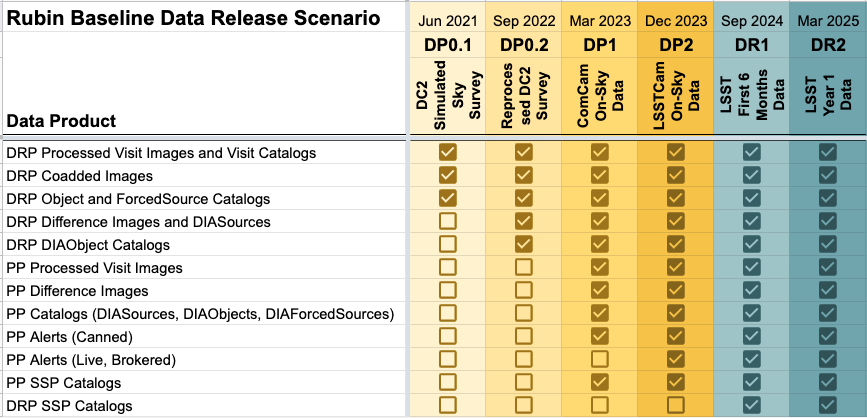
\includegraphics[width=\textwidth]{rubin_data_release_scenarios.png}
\end{figure}

% Include all the relevant bib files.
% https://lsst-texmf.lsst.io/lsstdoc.html#bibliographies
\section{References} \label{sec:bib}
\renewcommand{\refname}{} % Suppress default Bibliography section
\bibliography{local,lsst,lsst-dm,refs_ads,refs,books}

% Make sure lsst-texmf/bin/generateAcronyms.py is in your path
\section{Acronyms} \label{sec:acronyms}
\addtocounter{table}{-1}
\begin{longtable}{p{0.145\textwidth}p{0.8\textwidth}}\hline
\textbf{Acronym} & \textbf{Description}  \\\hline

CBP & Collimated Beam Projector \\\hline
ComCam & The commissioning camera is a single-raft, 9-CCD camera that will be installed in LSST during commissioning, before the final camera is ready. \\\hline
DP0 & Data Preview 0 \\\hline
DP1 & Data Preview 1 \\\hline
DP2 & Data Preview 2 \\\hline
DR1 & Data Release 1 \\\hline
FTE & Full-Time Equivalent \\\hline
LPM & LSST Project Management (Document Handle) \\\hline
LSST & Legacy Survey of Space and Time (formerly Large Synoptic Survey Telescope) \\\hline
NIR & Near Infrared \\\hline
OSI & open systems interconnect \\\hline
PDF & Portable Document Format \\\hline
PSF & Point Spread Function \\\hline
QA & Quality Assurance \\\hline
RDO & Rubin Directors Office \\\hline
SCOC & Survey Cadence Optimization Committee \\\hline
SE & System Engineering \\\hline
SIT & System Integration, Test \\\hline
SLAC & SLAC National Accelerator Laboratory \\\hline
US & United States \\\hline
\end{longtable}

% If you want glossary uncomment below -- comment out the two lines above
%\printglossaries



\end{document}
